\documentclass[11pt]{article}

\usepackage[utf8]{inputenc} 
\usepackage[T1]{fontenc} 
\usepackage{mathpazo} 
\usepackage{abstract}
\usepackage{graphicx} 
\usepackage{amsmath}
\begin{document}

%----------------------------------------------------------------------------------------
%	TITLE PAGE
%----------------------------------------------------------------------------------------

\begin{titlepage} 


	
	\newcommand{\HRule}{\rule{\linewidth}{0.5mm}} 
	
	\center
	
	%------------------------------------------------
	%	Headings
	%------------------------------------------------
	

	
	\textsc{\LARGE Szkoła Główna Gospodarstwa Wiejskiego}\\[2cm] 
	
	%------------------------------------------------
	%	Title
	%------------------------------------------------
	
	\HRule\\[0.4cm]
	
	{\huge\bfseries Zależność średnich wyników Polskich matur od województw}\\[0.4cm] 
	
	\HRule\\[1.5cm]
	
	%------------------------------------------------
	%	Author(s)
	%------------------------------------------------
	
	\begin{minipage}{0.4\textwidth}
		\begin{flushleft}
			\large
			\textit{Autorzy}\\
			O. \textsc{Deviatkin} \\
			K. \textsc{Kochański} \\
			R. \textsc{Kuligowski} \\
			M. \textsc{Laszczka} \\
			P. \textsc{Majewski} \\
		\end{flushleft}
	\end{minipage}
	~
	\begin{minipage}{0.4\textwidth}
		\begin{flushright}
			\large
			\textit{Prowadzący}\\
			Dr. Konrad \textsc{Furmańczyk} 
		\end{flushright}
	\end{minipage}
	
	% If you don't want a supervisor, uncomment the two lines below and comment the code above
	%{\large\textit{Author}}\\
	%John \textsc{Smith} % Your name
	
	%------------------------------------------------
	%	Date
	%------------------------------------------------

	



	
	%------------------------------------------------
	%	Logo
	%------------------------------------------------
	
	%\vfill\vfill
	%\includegraphics[width=0.2\textwidth]{placeholder.jpg}\\[1cm] % Include a department/university logo - this will require the graphicx package
	 
	%----------------------------------------------------------------------------------------
	

	\vspace*{\fill}
	{Warszawa 2022 } % Date, change the \today to a set date if you want to be precise
\end{titlepage}

%----------------------------------------------------------------------------------------


\section{Wstęp}
%	Tutaj opiszemu o co nam w ogóle chodzi
\section{Wyniki badań porównawczych }
%	Tutaj opiszemu wyniki
\begin{figure}[ht]
\resizebox{10cm}{!}{
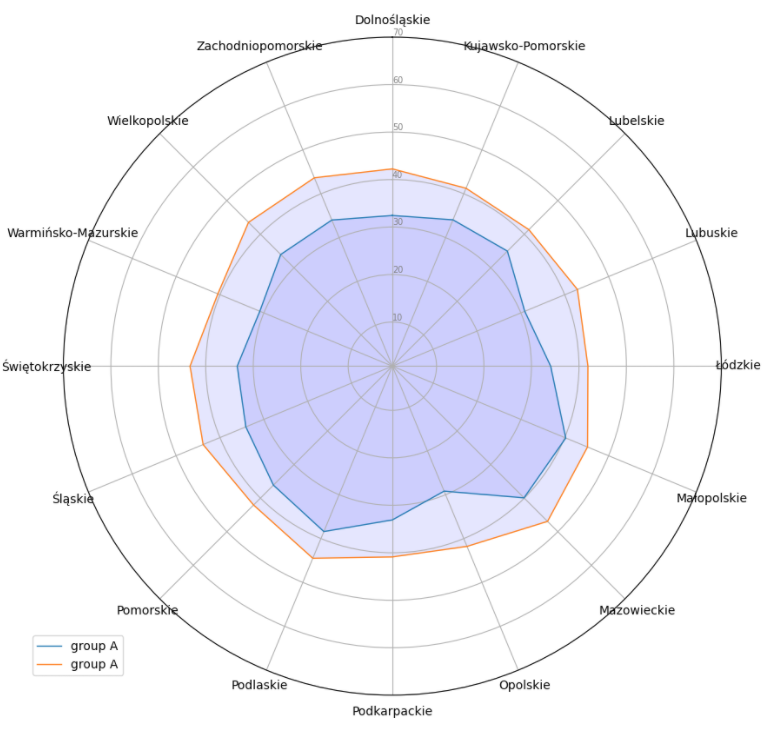
\includegraphics{obrazek.png}
}
\end{figure}
\begin{table}[h] % <-- note the [h]
\begin{center}
\begin{tabular}{|r|l|}\hline
Name & E-mail\\ \hline\hline
Michael Gustafson asdf sadf asd & mrg@duke.edu\\ \hline
Michael Ehrenfriedasdf sadf & mje7@duke.edu\\ \hline
\end{tabular}
\caption{\label{table:one}Caption Text} % <-- caption & label
\end{center}
\end{table}
This will now be referred to as Table \ref{table:one} on % <-- ref to table
page \pageref{table:one}. % <-- pageref
I can also say that Table \ref{table:one} is in Section
\ref{section:tl} because I put a label command in the % <-- ref to section
section title.

asd\\
asd\\
as\\
da\\
sd\\
asd\\
asd\\
\begin{figure}[ht]
\resizebox{10cm}{!}{
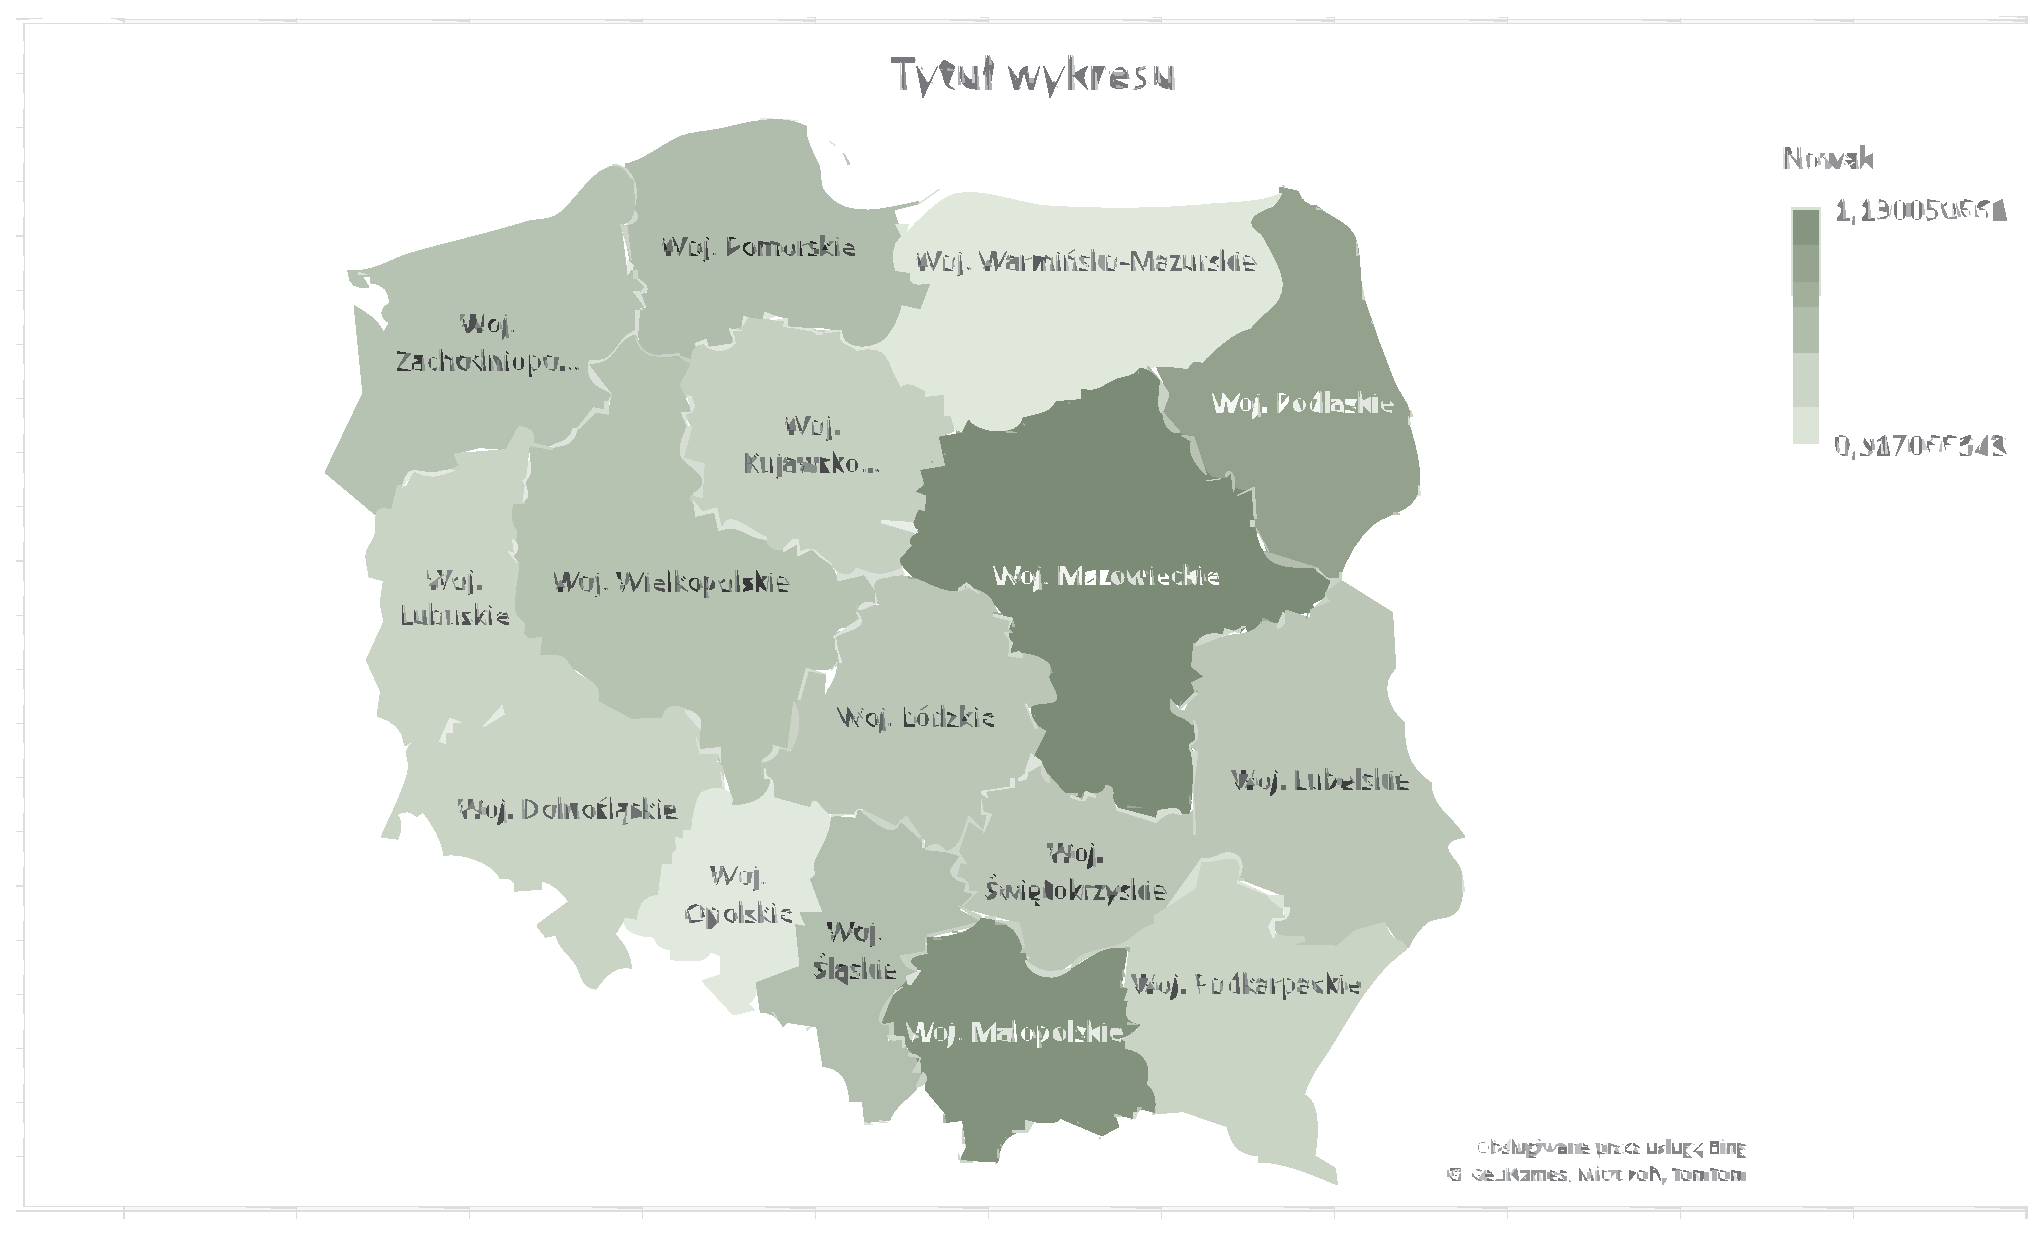
\includegraphics{obrazek2.eps}
}
\end{figure}
\section{Podsumowanie}
%	Tutaj opiszemu wnioski
\section{Literatura}
%	Tutaj opiszemu literature




\end{document}
